\section{Method Description}

\subsection{Coverage formula}

Here we proceed with the development of formula for computing the coverage value $c$ an intersecting shape boundary induces on a pixel. The intersecting portion of the border is assumed to be a straight line. The line is given by the signed distance $d$~to the center of the pixel and an attack angle $\phi$, which a perpendicular line through the center creates with the horizontal axis. Negative $d$ indicates that the center is inside the shape.

The pixel is a square with a side of length 1. Therefore, the result $c \in [0, 1]$ is defined as the area of the covered portion. The range of possible $d$ values varies for different~$\phi$, however, the widest range of $[-\frac{\sqrt{2}}{2}, \frac{\sqrt{2}}{2}]$ is achieved for angles $\phi = \frac{2k + 1}{4} \pi$.

First we find the value of $c(\phi, d)$ for $0 \leq \phi \leq \tquarterpi$ and $d \geq 0$. Other arguments are handled using
\begin{equation}
    c(\phi, -d) = 1 - c(\phi, d),
\end{equation}
and 8-way symmetry:
\begin{equation}
    c(\phi + \tfrac{k}{4}\pi, d) = \begin{cases}
    	c(              \phi, d), & k \equiv 0 \mod 2, \\
        c(\tquarterpi - \phi, d), & k \equiv 1 \mod 2.
    \end{cases}
\end{equation}

\begin{figure}\label{fig:coverage-formula}
	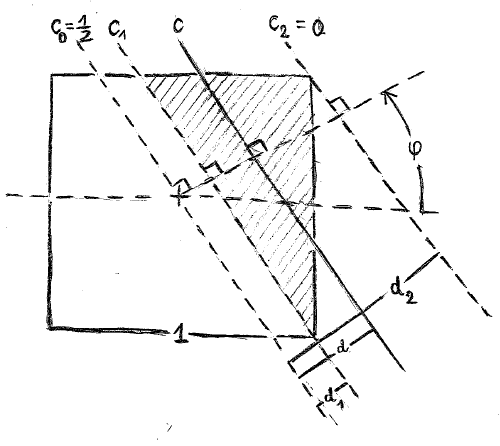
\includegraphics[width=8cm]{img/coverage-formula.png}
    \caption{Obtaining coverage induced by a half-plane}
\end{figure}

For a given angle $\phi$ Figure \ref{fig:coverage-formula} depicts the transition distance $d_1$ where the border passes a corner of the pixel square. Maximal distance $d_2$ is the the point beyond which the pixel stays completely outside. The coverage value $c_1 = c(\phi, d_1)$ is equal to the area of the single hatched triangle. Simple geometric inspection gives
\begin{equation}\begin{split}
	d_1 &= \tfrac{\sqrt{2}}{2}\cos(\tquarterpi + \phi), \\
    d_2 &= \tfrac{\sqrt{2}}{2}\cos(\tquarterpi - \phi), \\[3pt]
    c_1 &= \thalf \tan\phi.
\end{split}\end{equation}

When $d$ is between 0 and $d_1$, the coverage changes linearly from $\thalf$ to $c_1$. After that it falls toward 0 in a quadratic fashion until $d = d_2$. This observation leads to the following formula for the first octant:
\begin{equation}\label{eq:octant-coverge-formula}
	c(\phi, d) = \begin{cases}
    	\thalf + \frac{d}{d_1} \left( c_1 - \thalf \right),
        	& 0 \leq d < d_1, \\[6pt]
        \left(\frac{d_2 - d}{d_2 - d_1}\right)^2 c_1,
        	& d_1 \leq d < d_2.
	\end{cases}
\end{equation}
Obviously $c(\phi, d) = 0$ for $d \geq d_2$. Also notice that conservatively choosing the linear formula to be applied in range $[0, d_1)$, that is, with strict inequality at $d_1$,~prevents division by zero. This is an important detail when translating into numeric implementation. Figure \ref{fig:coverage-plot} shows a plot of $c(\phi, d)$ for selected values of $\phi$ with $d$~varying inside $[-d_2, d_2]$.

\begin{figure}\label{fig:coverage-plot}
	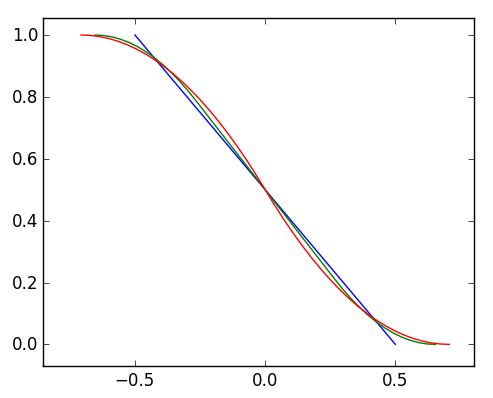
\includegraphics[width=8cm]{img/coverage-plot.png}
    \caption{Coverage value for different attack angles and varying distance}
\end{figure}